\documentclass[tikz,border=10pt]{standalone}
\usepackage[most]{tcolorbox}
\tcbuselibrary{listings}
\usetikzlibrary{arrows.meta}
\usetikzlibrary{calc}

\tcbuselibrary{skins}

% Define custom pastel colors
\definecolor{pastelblue}{RGB}{173,216,230}
\definecolor{pastelyellow}{RGB}{255,253,208}
\definecolor{pastelpink}{RGB}{255,209,220}
\definecolor{pastelgreen}{RGB}{176,226,172}
\definecolor{pastellavender}{RGB}{230,230,250}

\newtcolorbox{pastelbox}[2][]{
  enhanced,
  title=#2,
  colback=pastelblue!40,
  colframe=pastelblue!50,
  coltitle=pastelpink!70!black,
  fonttitle=\bfseries,
  colbacktitle=pastelpink!60,
  #1
}

\tikzset{every node/.style={inner sep=0pt}}


\begin{document}
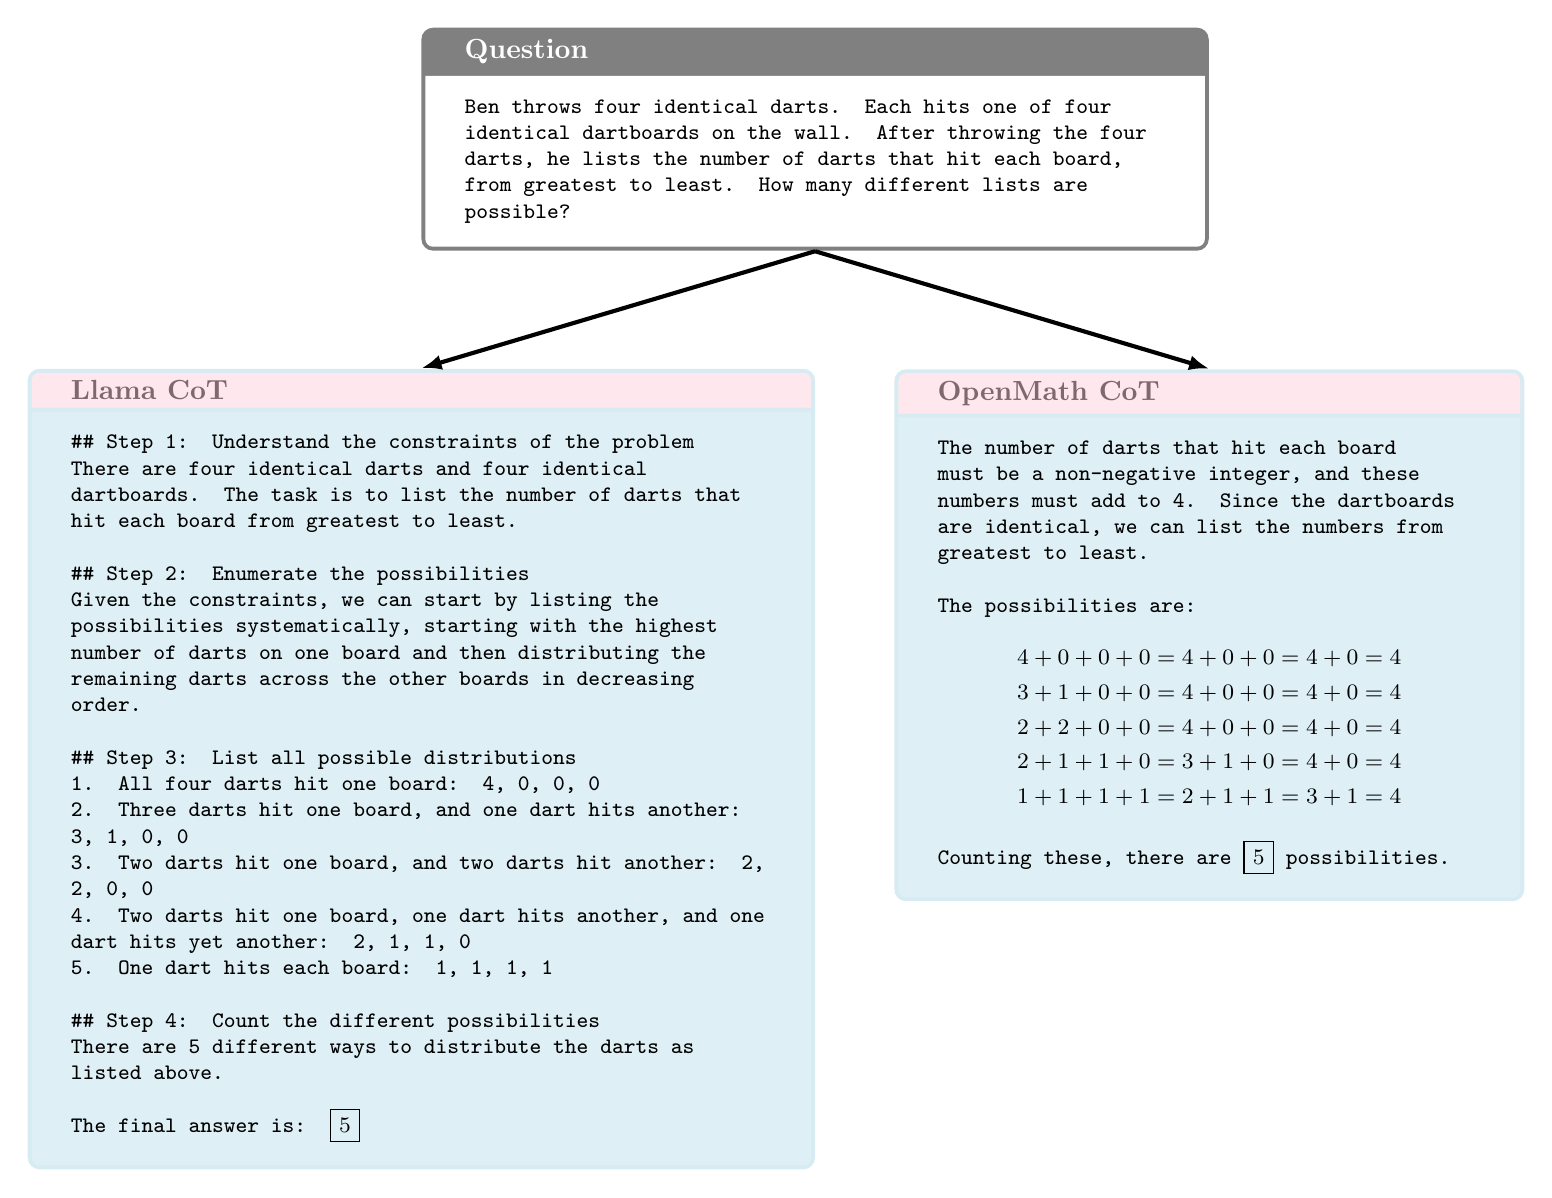
\begin{tikzpicture}
    % First tcolorbox (top middle)
    \node (box1) at (0,8) {
        \begin{tcolorbox}[
            width=10cm, 
            colback=white, 
            colframe=black!50,
            listing options={language=},
            fonttitle=\bfseries,
            fontupper=\ttfamily,
            title=Question
        ]
        % {Question}
            \footnotesize

Ben throws four identical darts. Each hits one of four identical dartboards on the wall. After throwing the four darts, he lists the number of darts that hit each board, from greatest to least.  How many different lists are possible?
        \end{tcolorbox}
    };
    
    % Second tcolorbox (bottom left)
    \node (box2) at (-5,0) {
        \begin{tcolorbox}[
            width=10cm, 
            colback=pastelblue!40,
            colframe=pastelblue!50,
            coltitle=pastelpink!50!black,
            colbacktitle=pastelpink!50,
            listing options={language=},
            fonttitle=\bfseries,
            fontupper=\ttfamily,
            title=Llama CoT,
        ]
\footnotesize

\#\# Step 1: Understand the constraints of the problem\\
There are four identical darts and four identical dartboards. The task is to list the number of darts that hit each board from greatest to least.\\\\
\#\# Step 2: Enumerate the possibilities\\
Given the constraints, we can start by listing the possibilities systematically, starting with the highest number of darts on one board and then distributing the remaining darts across the other boards in decreasing order.\\\\
\#\# Step 3: List all possible distributions\\
1. All four darts hit one board: 4, 0, 0, 0\\
2. Three darts hit one board, and one dart hits another: 3, 1, 0, 0\\
3. Two darts hit one board, and two darts hit another: 2, 2, 0, 0\\
4. Two darts hit one board, one dart hits another, and one dart hits yet another: 2, 1, 1, 0\\
5. One dart hits each board: 1, 1, 1, 1\\\\
\#\# Step 4: Count the different possibilities\\
There are 5 different ways to distribute the darts as listed above.\\\\
The final answer is: $\boxed{5}$       
\end{tcolorbox}
    };
    
    % Third tcolorbox (bottom right)
    \node (box3) at ($(box2.east)+(5,1.7)$) {
    % (5,box2.north ) {
        \begin{tcolorbox}[
            width=8cm, 
            colback=pastelblue!40,
            colframe=pastelblue!50,
            coltitle=pastelpink!50!black,
            colbacktitle=pastelpink!50,
            listing options={language=},
            fonttitle=\bfseries,
            fontupper=\ttfamily,
            title=OpenMath CoT
        ]
        \footnotesize
The number of darts that hit each board must be a non-negative integer, and these numbers must add to 4. Since the dartboards are identical, we can list the numbers from greatest to least.\\\\
The possibilities are:\\
\[ 4 + 0 + 0 + 0 = 4 + 0 + 0 = 4 + 0 = 4 \] 
\[ 3 + 1 + 0 + 0 = 4 + 0 + 0 = 4 + 0 = 4 \] 
\[ 2 + 2 + 0 + 0 = 4 + 0 + 0 = 4 + 0 = 4 \] 
\[ 2 + 1 + 1 + 0 = 3 + 1 + 0 = 4 + 0 = 4 \] 
\[ 1 + 1 + 1 + 1 = 2 + 1 + 1 = 3 + 1 = 4 \]\\
% Counting these, there are \$\boxed{5}\$ possibilities.
Counting these, there are $\boxed{5}$ possibilities.
        \end{tcolorbox}
    };
    
    \draw[-{Latex[scale=0.75]}, line width=1.5pt] (box1.south) -- (box2.north);

    \draw[-{Latex[scale=0.75]}, line width=1.5pt] (box1.south) -- (box3.north);

\end{tikzpicture}
\end{document}
